\documentclass{beamer}

\usetheme[]{boxes}
%\usetheme[]{CambridgeUS}
%\usetheme[]{Singapore}
%\usetheme[]{Boadilla}
\usefonttheme[onlylarge]{structurebold}
\setbeamerfont*{frametitle}{size=\normalsize,series=\bfseries}
\setbeamertemplate{navigation symbols}{}
\useinnertheme{circles}
\usecolortheme{fly}
%\useoutertheme[footline=empty]{miniframes}
%\setbeamercolor{normal text}{bg=black!20}

\usepackage[english]{babel}
\usepackage{ucs}
\usepackage[utf8x]{inputenc}
\usepackage[T1]{fontenc}
\usepackage{hyperref}
\renewcommand{\rmdefault}{pad}
\renewcommand{\sfdefault}{pfr}
\usepackage{textpos}

% Setup TikZ

\usepackage{tikz}
\usetikzlibrary{arrows}
\tikzstyle{block}=[draw opacity=0.7,line width=1.4cm]

\title[Time and Reciprocity]
{%
  Time and Reciprocity in Improvisation
}
\subtitle[In-time performance]
{%
  On the aspect of in-time systems in improvisation with and on machines.
}
\author{Henrik Frisk}

\institute[Lund University]
{
  Malmoe Academy of Music, Lund University
}
\date{EarZoom 2010, Ljubljana}

\begin{document}

\begin{frame}
  \titlepage
\end{frame}


%%%%%%%%%%%%%%%%%%%%%%%%%%%%%%
% Thesis
%%%%%%%%%%%%%%%%%%%%%%%%%%%%%%
\begin{frame}
  \frametitle{PhD Thesis}
  \begin{center}
    \includegraphics[width=.3\textwidth]{img/imp-comp-int.png}
    % 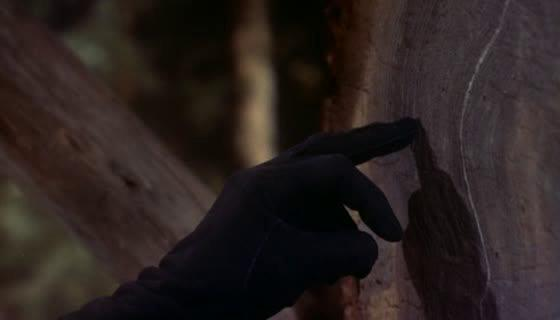
\includegraphics[width=.8\textwidth]{media/vertigo-finger.jpg}
  \end{center}
  \begin{center}
    \emph{Improvisation, Computers, and Interaction: Rethinking Human-Computer Interaction Through Music}
  \end{center}
  \uncover<2->{
    \begin{center}
      (\url{www.performingarts.lu.se})
    \end{center}
  }
\end{frame}

%%%%%%%%%%%%%%%%%%%%%%%%%%%%%%
% CD
%%%%%%%%%%%%%%%%%%%%%%%%%%%%%%
\begin{frame}
  \frametitle{etherSound CD}
  \begin{center}
    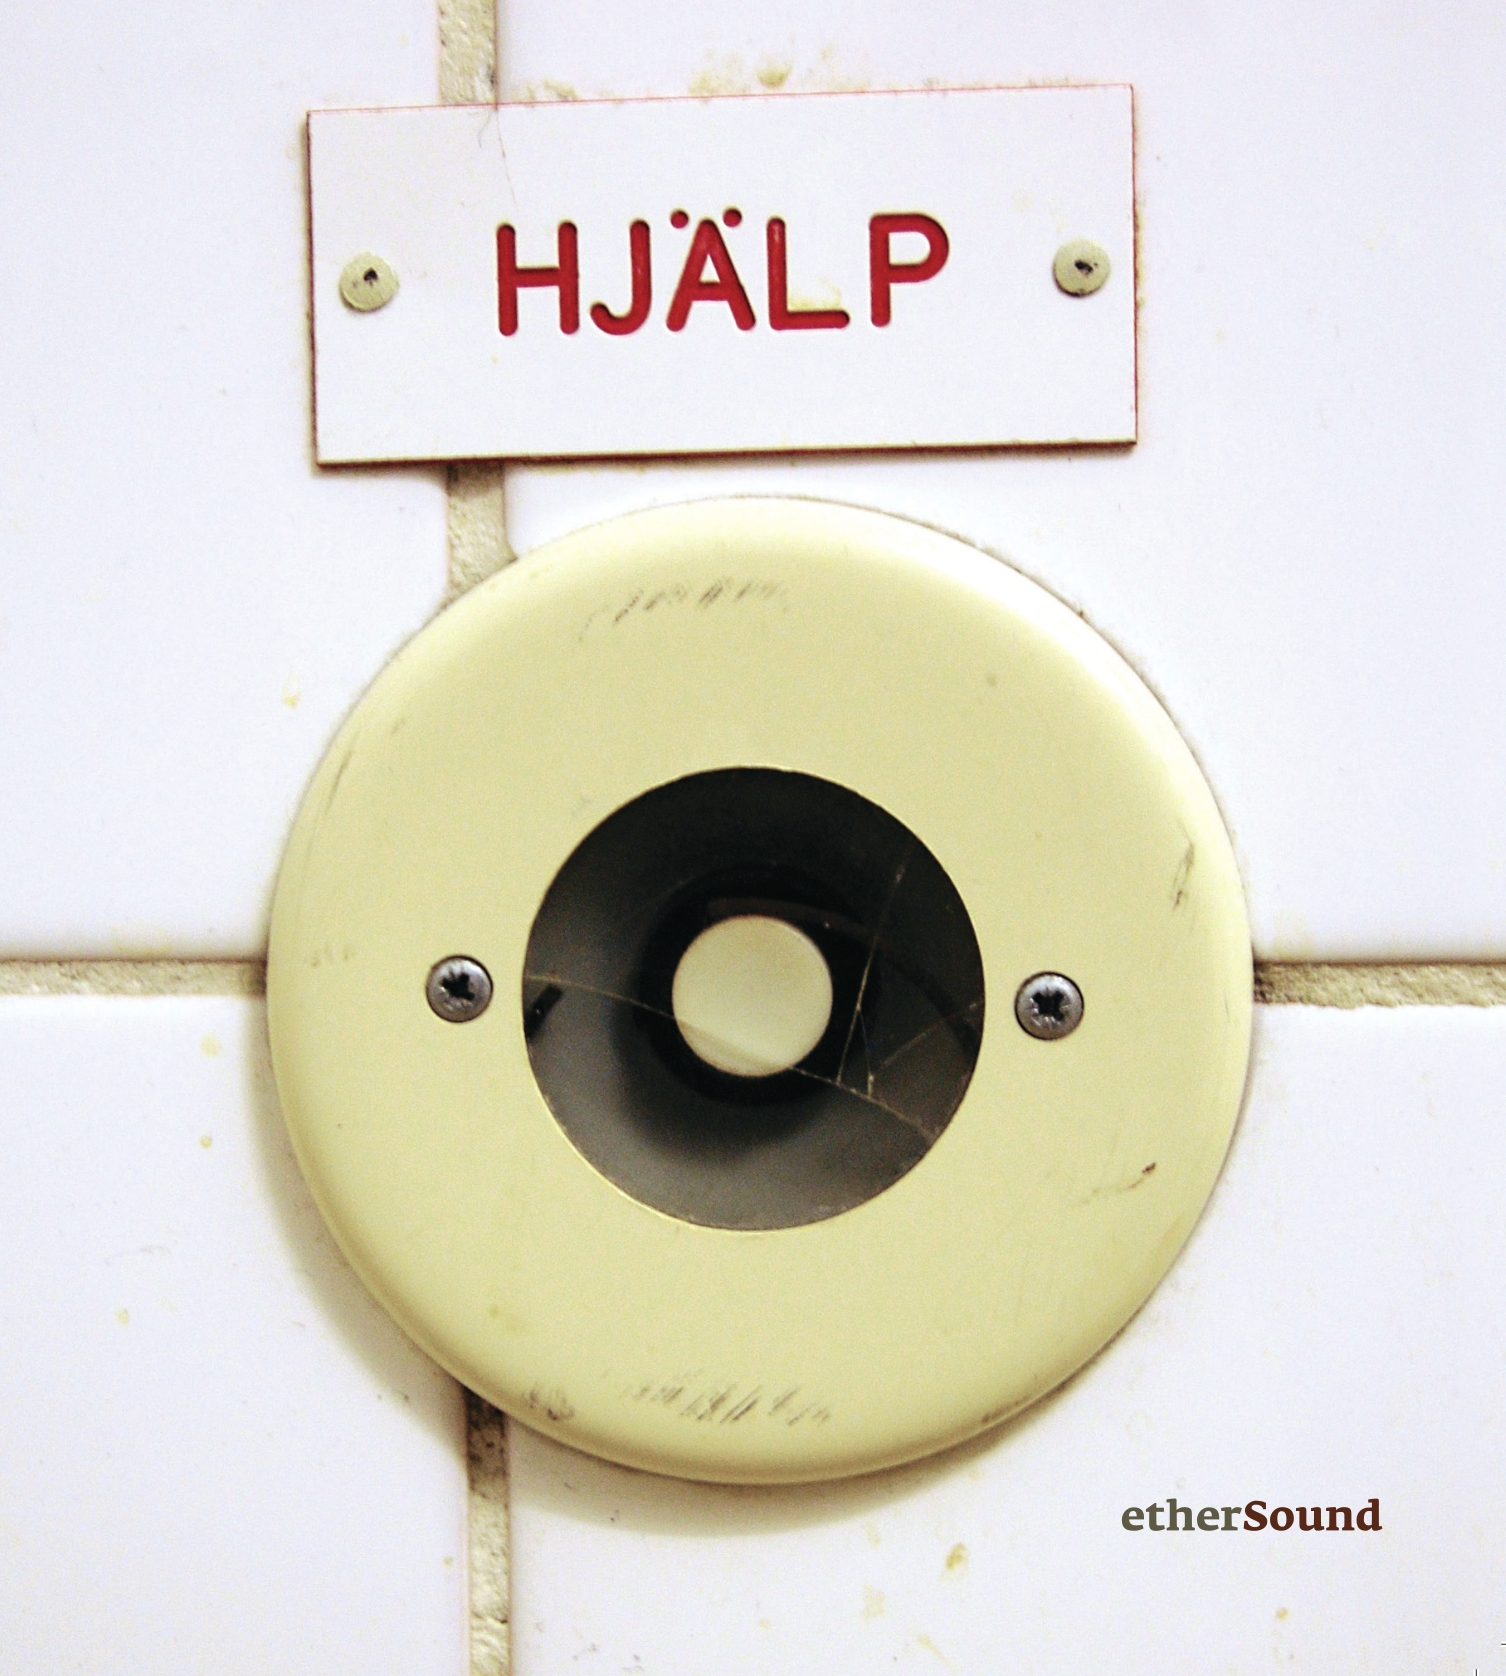
\includegraphics[width=.4\textwidth]{img/ether-cover.jpg}
    % 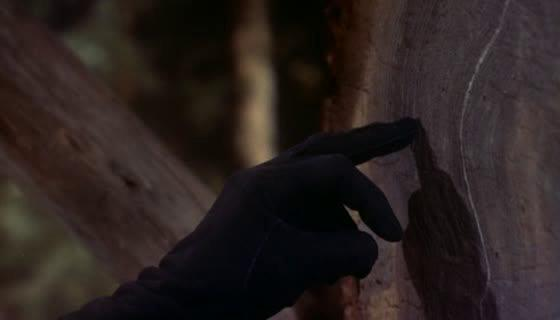
\includegraphics[width=.8\textwidth]{media/vertigo-finger.jpg}
  \end{center}
  \uncover<2->{
    \begin{center}
      \url{www.kopasetic.se}
    \end{center}
  }
  \uncover<3->{  
    \begin{center}
      \url{www.henrikfrisk.com}
    \end{center}
  }
\end{frame}

%%%%%%%%%%%%%%%%%%%%%%%%%%%%%%
% Ny book
%%%%%%%%%%%%%%%%%%%%%%%%%%%%%%
\begin{frame}
  \frametitle{New book}
  \begin{center}
    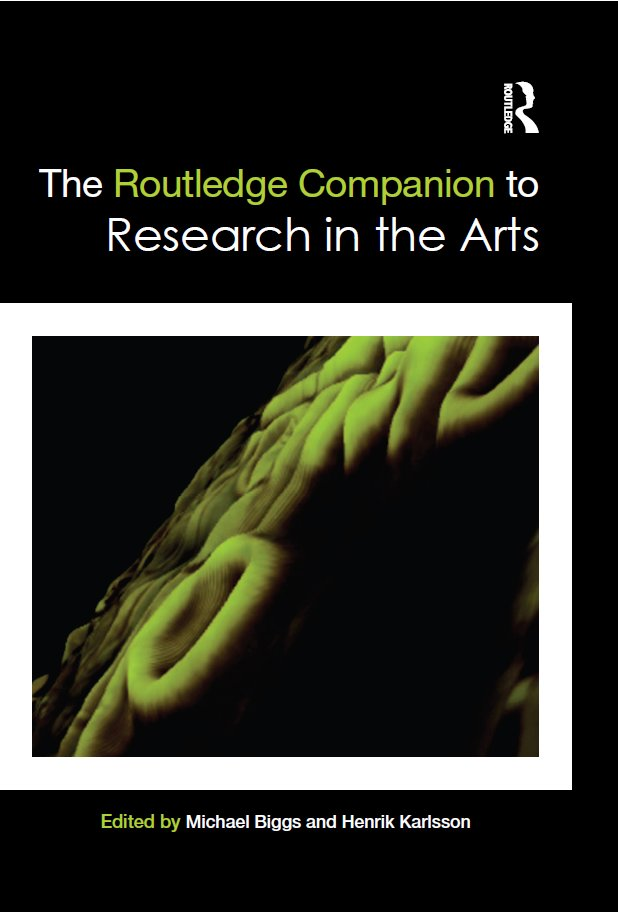
\includegraphics[width=.4\textwidth]{img/research-in-the-arts.jpg}
    % 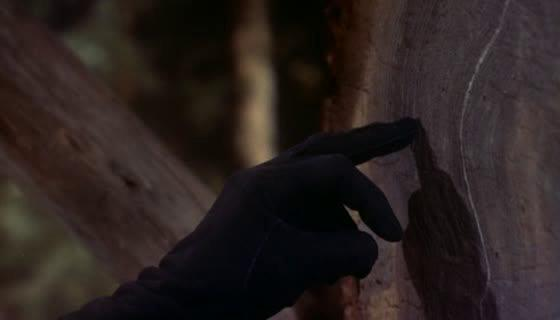
\includegraphics[width=.8\textwidth]{media/vertigo-finger.jpg}
  \end{center}
  % \begin{center}
  %   \emph{Improvisation, Computers, and Interaction: Rethinking Human-Computer Interaction Through Music}
  % \end{center}
\end{frame}

%%%%%%%%%%%%%%%%%%%%%%%%%%%%%%
% Different temporalities
%%%%%%%%%%%%%%%%%%%%%%%%%%%%%%
\begin{frame}
  \frametitle{Different temporalities}
  \begin{block}{Improvisation vs. Composition}
    \begin{itemize}
    \item <2->Improvised music unfolds in real-time.
    \item <3->Composition takes place in non-real-time
    \end{itemize}
  \end{block}
  \uncover<4->{\emph{The way improvisation is embedded in time is one of its significant features.}}
  \pause[5]
  \begin{block}{Machine vs. Human}
    \begin{itemize}
    \item <5->Machine temporality is different...
    \item <6->Computer instruments should be constructed taking the difference into consideration.
    \end{itemize}
  \end{block}
\end{frame}

%%%%%%%%%%%%%%%%%%%%%%%%%%%%%%
% Obvious differences?
%%%%%%%%%%%%%%%%%%%%%%%%%%%%%%
\begin{frame}
  \frametitle{Improvisation vs. Composition}
  \begin{block}{Obvious differences?}
    \begin{columns}
      \pause[2] \column{.6\textwidth}
      \includegraphics<1->[width=5cm]{img/repetition-excerpt.jpg} 
      \pause[3]
      \column{.4\textwidth}
      \includegraphics<1->[width=3cm]{img/action-painting.jpg}
    \end{columns}
  \end{block}
\end{frame}

\begin{frame}
  \begin{block}{Is a prepared improvisation not improvised?\vspace{.5cm}}
    \begin{columns}[t]
      \pause[2] \column{.4\textwidth}
    \begin{center}
      \includegraphics<1->[width=4cm]{img/bird.jpg}
    \end{center}
      \pause[3]
      \column{.6\textwidth}
      \begin{textblock}{6}(0,2)
        \emph{An improvisation is always constructed in real-time.}
      \end{textblock}
    \end{columns}
  \end{block}
\end{frame}

%%%%%%%%%%%%%%%%%%%%%%%%%%%%%%
% Non Real-Time or Real-Time
%%%%%%%%%%%%%%%%%%%%%%%%%%%%%%
\begin{frame}{
    \begin{center}
      Non Real-Time or Real-Time?
    \end{center}
  }
  \begin{columns}
        \pause[2] \column{.5\textwidth}
    \begin{center}
      \includegraphics<1->[width=3cm]{img/picasso.jpg}
    \end{center}
    \pause[3] \column{.5\textwidth}
    \begin{center}
      \includegraphics<2->[width=3cm]{img/bailey.jpg}
    \end{center}
  \end{columns}
\end{frame}

%%%%%%%%%%%%%%%%%%%%%%%%%%%%%%
% In-time vs Over-time graphics
%%%%%%%%%%%%%%%%%%%%%%%%%%%%%%
\begin{frame}
  \frametitle{Alternate distinction}
  \begin{columns}[t]
    \column{.5\textwidth}   
    \emph{In-time}
      \includegraphics<1->[width=2cm]{img/in-time.png}
    \pause[2] 
    \column{.5\textwidth}
    \emph{Over-time}
      \includegraphics<2->[width=2cm]{img/over-time.png}
  \end{columns}
\end{frame}

%%%%%%%%%%%%%%%%%%%%%%%%%%%%%%
% Bibliographic reference to Iyer
%%%%%%%%%%%%%%%%%%%%%%%%%%%%%%
\begin{frame}%{In-time vs over-time}
  \begin{thebibliography}{Vijay Iyer, 2008}
  \bibitem[Iyer, Vijay, 2008]{iyer08}
    V. Iyer (2008)
    \newblock `On improvisation, temporality, and embodied experience.'
    \newblock (Chapter~26 in \emph{Sound Unbound : Sampling digital music and culture}, (Paul~D. Miller, edito). The MIT Press, Cambridge, Mass., 2008.)
    
    \pause[2]
  \bibitem[Smithers, Tim, 1996]{smithers96}
    T. Smithers (1996)
    \newblock `On What Embodiment Might Have to do with Cognition.'
    \newblock (Tech report published by AAAI, 1996)
  \end{thebibliography}
\end{frame}

%%%%%%%%%%%%%%%%%%%%%%%%%%%%%%
% Constraints and allowances...
%%%%%%%%%%%%%%%%%%%%%%%%%%%%%%
\begin{frame}
  \frametitle{Constraints and allowances...}
  \begin{block}{Typical in-time operations}
    \begin{itemize}
    \item <2->Musical performance
    \item <3->Improvisation
    \end{itemize}
  \end{block}
  \pause[4]
  \begin{block}{Over-time operations}
    \begin{itemize}
    \item <5->Composition
    \item <6->Reading a book
    \item<7-> Computation
    \end{itemize}
    \uncover<8->{
      \begin{center}
        \emph{Real-time (computation) is not necessarily in-time:}
      \end{center}
    }
    \uncover<9->{
      \begin{center}
        \alert{Resistance is an integral part of in-time operations.}
      \end{center}
    }
  \end{block}
\end{frame}

%%%%%%%%%%%%%%%%%%%%%%%%%%%%%%
% What is interaction?
%%%%%%%%%%%%%%%%%%%%%%%%%%%%%%
\begin{frame}
  \frametitle{What is interaction?}
  \pause[2]
    \begin{block}{Problematic...}
      \begin{itemize}
      \item<3-> ``Reciprocally active'' (OED Online)
      \item<4-> In computer interface design: \uncover<4->{\alert{control}}
      \item<5-> In improvised music: \uncover<6->{\alert{exchange, communication and reciprocity} (see \emph{Saying Something} by Ingrid Monson (1996))}
      \end{itemize}
    \end{block}
\end{frame}

%%%%%%%%%%%%%%%%%%%%%%%%%%%%%%
% Differences
%%%%%%%%%%%%%%%%%%%%%%%%%%%%%%
\begin{frame}
  \frametitle{Musical interaction}
  \begin{block}{}
    \begin{columns}[t]
      \column{.4\textwidth}
      \begin{block}{Sensitivity}
        A succesful interplay between musicians rests on a mutual sensitivity
        for taking, and responding to, musical initiatives.
      \end{block}
      \pause[2] 
      \column{.4\textwidth}
      \begin{block}{Difference}
          Musicians induce differences that ``\emph{make a difference}'' and
          according to Gregory Bateson, such a difference that makes a
          difference is the definition of a bit of information (Bateson 1979, \emph{Mind and Nature})
      \end{block}
    \end{columns}
  \end{block}
\end{frame}

%%%%%%%%%%%%%%%%%%%%%%%%%%%%%%
% Bateson and beyond
%%%%%%%%%%%%%%%%%%%%%%%%%%%%%%
\begin{frame}
  \frametitle{Bateson and beyond}
  \pause[2]
  \begin{block}{}
    \begin{columns}[t]
      \column{.4\textwidth}
      \begin{block}{Interaction-as-control}
        \uncover<3->{Influences much of our interaction design.}
        % \includegraphics<2->[width=4cm]{img/tvset.png}
      \end{block}
      \column{.4\textwidth}
      \begin{block}{Interaction-as-difference}
        \uncover<4->{To exploit the constraints and allowances of the natural timescales of the technology used.}
      \end{block}
    \end{columns}
    \vspace{1cm}
    \uncover<5->{
      \begin{columns}[c]
        \column{.2\textwidth}click and\\response
        \column{.55\textwidth}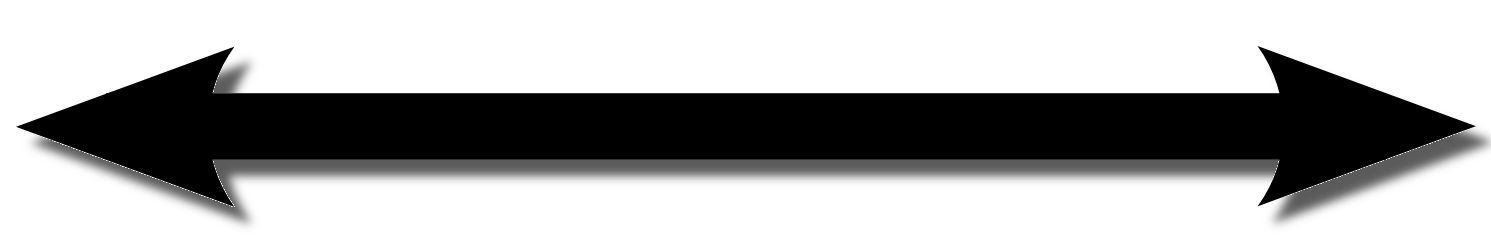
\includegraphics[width=.9\textwidth]{img/dbl-arrow.png}
        \column{.2\textwidth}musical\\interaction
      \end{columns}
    }
  \end{block}
\end{frame}

%%%%%%%%%%%%%%%%%%%%%%%%%%%%%%
% The interactive continuum
%%%%%%%%%%%%%%%%%%%%%%%%%%%%%%
\begin{frame}
  \frametitle{The interactive continuum}
    \uncover<1->{
      \begin{columns}[c]
        \column{.2\textwidth}click and\\response
        \column{.55\textwidth}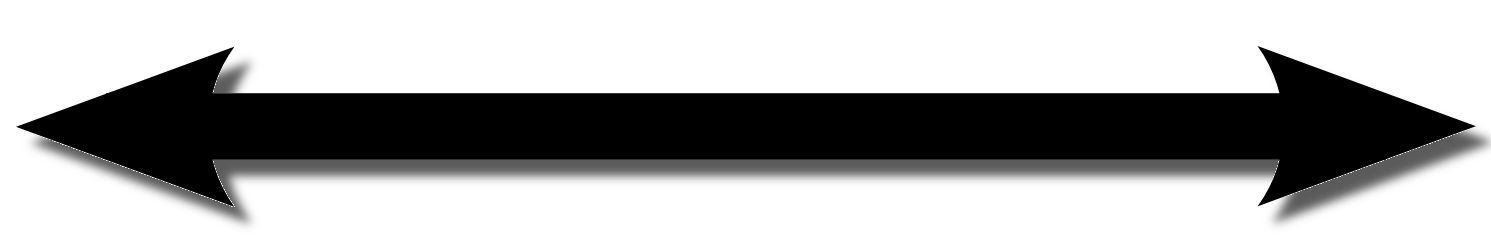
\includegraphics[width=.9\textwidth]{img/dbl-arrow.png}
        \column{.2\textwidth}musical\\interaction
      \end{columns}
    }
  \vspace{1cm}
    \uncover<2->{
      \begin{columns}[c]
        \column{.2\textwidth}control
        \column{.55\textwidth}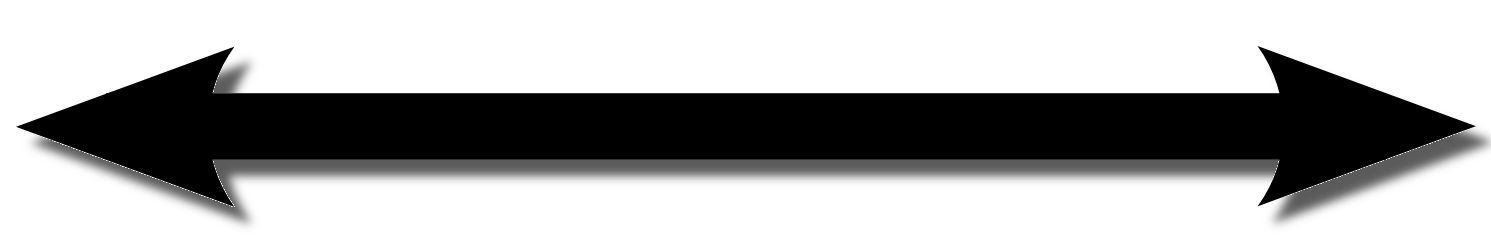
\includegraphics[width=.9\textwidth]{img/dbl-arrow.png}
        \column{.2\textwidth}influence over content
      \end{columns}
    }
\end{frame}

%%%%%%%%%%%%%%%%%%%%%%%%%%%%%%
% Multiple temporalities
%%%%%%%%%%%%%%%%%%%%%%%%%%%%%%
\begin{frame}
  \frametitle{Multiple temporalities}
  \pause[2]
  \begin{block}{}
    \begin{itemize}
    \item<2-> Curtis Roads: perceptual discontinuities in the boundaries between different time scales.
    \item<3-> Stockhausen: the time spectrum of a fundamental duration.
    \item<3-> Xenakis:
      \begin{itemize}\item<4-> the discontinuity of musical time and multiple time scales\ldots
      \item<5-> \ldots and of time to space transformations.
      \end{itemize}
    \end{itemize}
  \end{block}
  \pause[6]
  \begin{block}{}
    \emph{Time to space transformation is a recurring thread in several art forms.}
  \end{block}
\end{frame}

%%%%%%%%%%%%%%%%%%%%%%%%%%%%%%
% Vertigo
%%%%%%%%%%%%%%%%%%%%%%%%%%%%%%
\begin{frame}
  \frametitle{Vertigo (Hitchcock 1959)}
  \begin{center}
    \href{run:media/vertigo-test.avi}{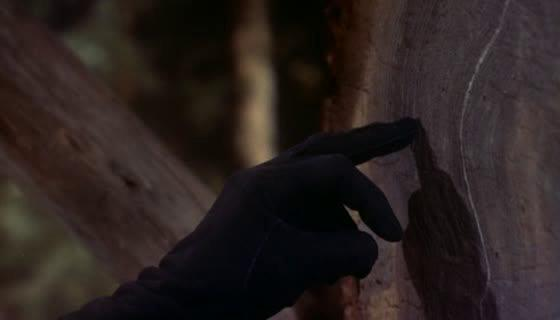
\includegraphics[width=.8\textwidth]{media/vertigo-finger.jpg}}
    % 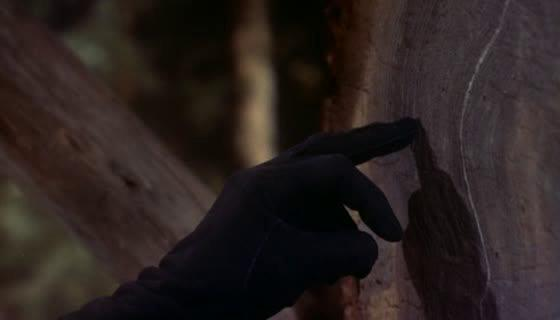
\includegraphics[width=.8\textwidth]{media/vertigo-finger.jpg}
  \end{center}
  \begin{center}
    \emph{``It was only a moment to you...''}
  \end{center}
\end{frame}

%%%%%%%%%%%%%%%%%%%%%%%%%%%%%%
% Wagner
%%%%%%%%%%%%%%%%%%%%%%%%%%%%%%
\begin{frame}
  \frametitle{Parsifal (Wagner)}
  \begin{center}
    \href{run:media/Parsifal.mp4}{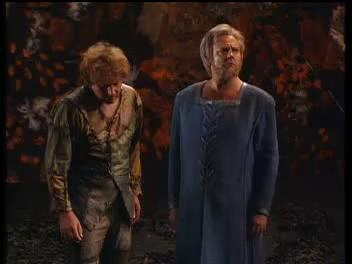
\includegraphics[width=.6\textwidth]{media/parsifal-splash.jpg}}
    % 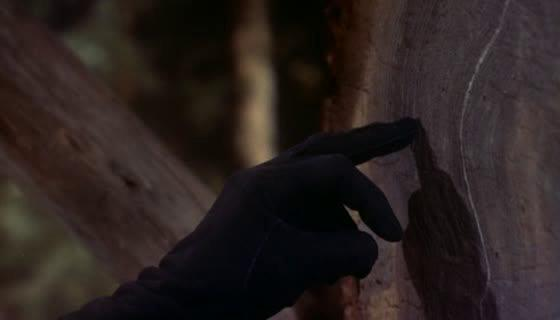
\includegraphics[width=.8\textwidth]{media/vertigo-finger.jpg}
  \end{center}
  \begin{center}
    \emph{``Du siehst, mein Sohn, zum Raum wird hier Zeit.''}
  \end{center}
\end{frame}

%%%%%%%%%%%%%%%%%%%%%%%%%%%%%%
% The spatial representation of music
%%%%%%%%%%%%%%%%%%%%%%%%%%%%%%
\begin{frame}
   \frametitle{The spatial representation of music}
   \pause[2]
   \begin{block}{}
     \begin{itemize}
     \item<2-> Musical notation is the out-of-time representation of music.
     \item<3-> What constitutes music?
       \begin{itemize}
       \item<4-> What we experience in the sounds, or\ldots
       \item<5-> \ldots what we might appreciate of the score? (Wishart 1996)
       \end{itemize}
     \item<6-> A recording is a spatial representation. (Evens 2005)
     \item<7-> The digital representation of sound is similarily (abstractly) spatialized. 
     \end{itemize}
   \end{block}
   \uncover<8->{
     \begin{block}{}
     \emph{To even begin to think about using interactive computer technology
       in performance involves a transformation of the in-time embedded sound
       to an over-time representation.}
   \end{block}
 }
\end{frame}

%%%%%%%%%%%%%%%%%%%%%%%%%%%%%%
% Lack of liveness?
%%%%%%%%%%%%%%%%%%%%%%%%%%%%%%
\begin{frame}
  \frametitle{Lack of `liveness' in digital performance}
  \begin{columns}
    \uncover<1->{    
      \column{.45\textwidth}
      \begin{center}
        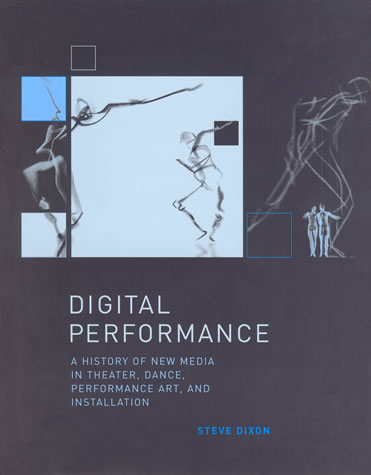
\includegraphics[width=.9\textwidth]{img/digital-perf.jpg}
      \end{center}
    }
    \column{.5\textwidth}
    \uncover<2->{    \begin{block}{}
      \begin{itemize}
      \item<2-> Realtime art becomes less live when technology is used?
      \item<3-> Computers disrupt the in-time processes of performance?
      \item<4-> Why?
        \begin{itemize}
        \item<5-> Poor interaction design?
        \item<6-> Limitied understanding for the in-time prerequisites?
        \end{itemize}
      \end{itemize}
    \end{block}
}  \end{columns}
\end{frame}

%%%%%%%%%%%%%%%%%%%%%%%%%%%%%%
% Summary
%%%%%%%%%%%%%%%%%%%%%%%%%%%%%%
\begin{frame}
  \frametitle{Summary}
  \pause[2]
  \begin{block}{}
    \begin{itemize}
    \item<2-> The use of computers in artistic practice highlights questions
      relating to in-time interaction makes the practice both artistically and
      conceptually interesting.
    \item<3-> Knowledge produced about the interaction and about the ways in
      which it may be improved, may well be of interest also outside of that
      field of art practicies.
    \end{itemize}
  \end{block}
  \pause[4]
  \begin{block}{}
    \begin{itemize}
    \item<4-> To more fully understand the notion of liveness and temporal
      embeddedness in the real-time arts involving computers.
    \item<5-> May be used inform the design of new human-computer interfaces.
    \end{itemize}
  \end{block}
\end{frame}

%%%%%%%%%%%%%%%%%%%%%%%%%%%%%%
% Thank you
%%%%%%%%%%%%%%%%%%%%%%%%%%%%%%
\begin{frame}
   \frametitle{}
   \begin{block}{Thank you.}
     \begin{center}
       \huge{?}
     \end{center}
   \end{block}
   \begin{textblock}{7}(-1,2)
     
\includegraphics[width=\textwidth]{img/mhm-logo}
%     Test
   \end{textblock}
\end{frame}

\end{document}
